\documentclass[11pt]{beamer}
\usepackage{verbatim}
\usepackage{amsmath}
\usepackage{amsthm}
\usepackage{graphics}
\usepackage{multicol}
\usepackage{color}
\usepackage{stmaryrd}\usefonttheme[onlymath]{serif}

\title{Progress Report 1: Code Generation}
\date{\today}
\author{Xie Li}
\begin{document}
\maketitle

\begin{frame}\frametitle{Overview of the Progress}
\begin{itemize}
\item Finish the refinement of the generated code and able to communicate once between alice and bob.

\item Begin to change the implementation of the code generation module based on the implementation.
\end{itemize}
\end{frame}

\begin{frame}\frametitle{Modeling}

\end{frame}

\begin{frame}\frametitle{Running Result}
\begin{multicols}{2}
\begin{center}
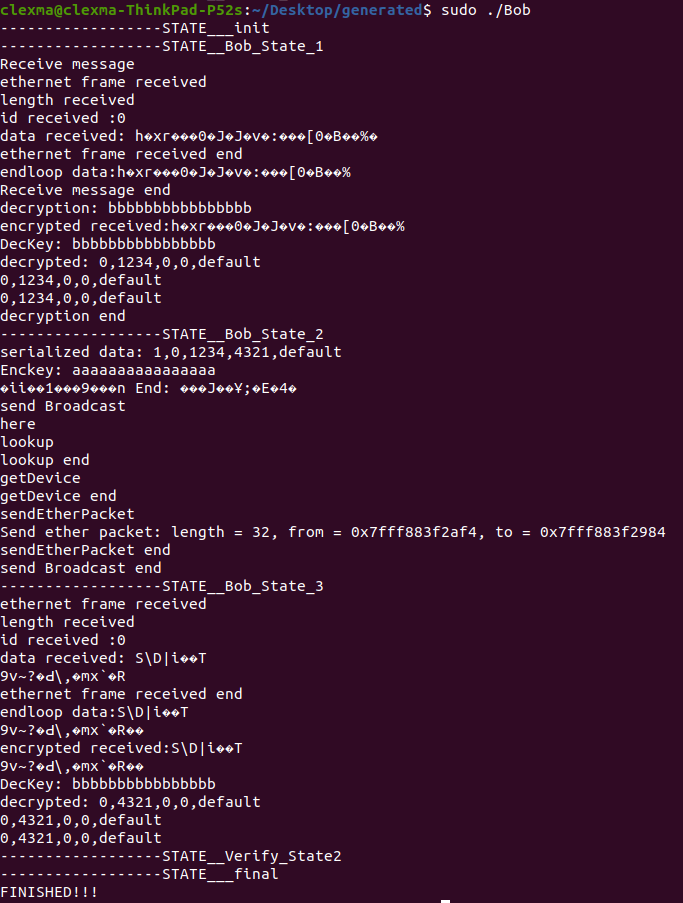
\includegraphics[scale=0.25]{bob.png}

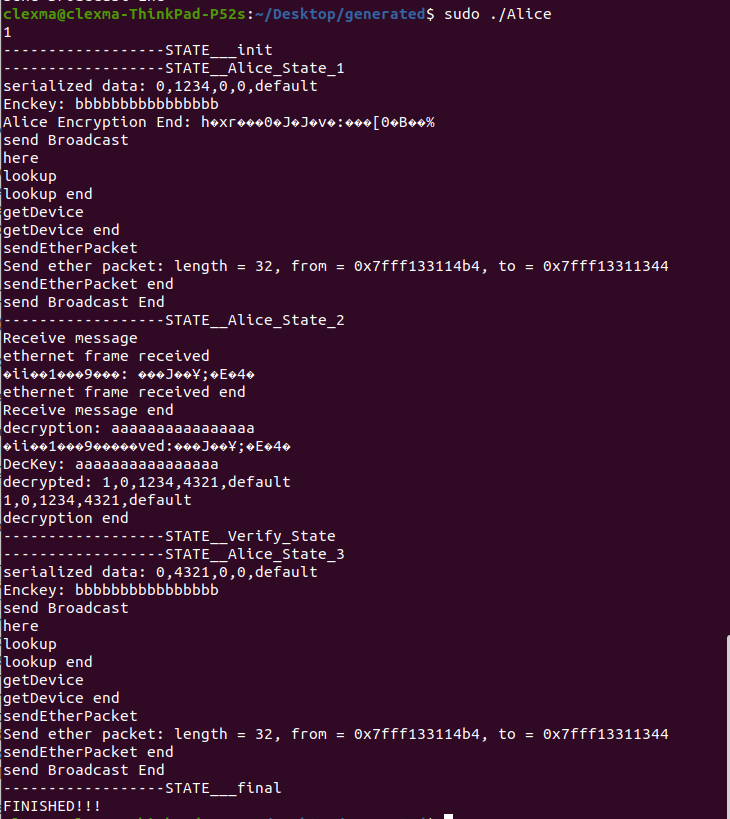
\includegraphics[scale=0.25]{alice.png}
\end{center}

\end{multicols}
\end{frame}

\begin{frame}\frametitle{Problems}
\begin{itemize}
\item Serialization $\rightarrow$ Encryption $\rightarrow$ Decryption $\rightarrow$ Deserialization(ERROR)

\item Identification of the package: currently the package are identified with the  id and ethernet protocol number 0x888f.

\item Length of the array when receiving.
\end{itemize}
\end{frame}

\begin{frame}\frametitle{Questions}
\begin{itemize}
\item How ``automatic'' should we be?

\end{itemize}
\end{frame}

\begin{frame}\frametitle{Later Work}
\begin{itemize}
\item An overall test combining different modules.
\begin{itemize}
\item UDP communication.
\item Other en/decryption algorithms.(Currently is AES).

\item Find new serialization library.(JSON based e.g.)
\end{itemize}

\item Refactor of the code generation module.
\begin{itemize}
\item Add the generation of compile code.
\item Refine the code related to cryptor and communicatio based on the refined generated code.
\item More functionalities?
\end{itemize}
\end{itemize}
\end{frame}
\end{document}